\chapter{Numerical applications}

\epigraph{The most obvious characteristic of science is its application: the fact that, as a consequence of science, one has a power to do things. And the effect this power has had need hardly be mentioned. The whole industrial revolution would almost have been impossible without the development of science.}{\textit{Richard Feynman \\ The Meaning of It All: Thoughts of a Citizen-Scientist}}
\minitoc

\lettrine{\color{theme}{T}}he proposed finite element discretization can be employed for different numerical applications. The chapter is organized as follows:
\begin{itemize}
	\item a boundary stabilization problem for the Kirchhoff plate and for the irrotational shallow water equations is presented in Sec. \secref{sec:bd_stab};
	\item Sec. \secref{sec:mixbd_enfor} presents a comparison of the Lagrange multiplier \ref{sec:lagrMul} and the virtual domain decomposition method \ref{sec:vdd} for the enforcement of mixed boundary conditions;
	\item a thermoelastic problem for which an analytic solution is avaiable is illustrated in Sec. \secref{sec:thelas_wave}.
\end{itemize}



\section{Boundary stabilization}\label{sec:bd_stab}

In this section, we consider the boundary stabilization of a cantilever Kirchhoff plate of the irrotational shallow water equations. For pHs a simple proportional gain assures asymptotic system of the system thanks to the LaSalle’ invariance principle \cite[chapter
6, proposition 6.2]{duindam2009}. This can be used to achieve stabilization of the undeformed configuration of the Kirchhoff plate. For the shallow water equation a reference is also added to stabilizes the system around a certain fluid height.


\subsection{Cantilever Kirchhoff plate}

\begin{figure}[t]
	\centering
	\includegraphics[width=0.5\textwidth]{part_3/applications/bs_Kirchh/plate_controlled.eps}
	\caption{Cantilever plate subjected to a control forces on the lateral sides.}
	\label{fig:plate_controlled}
\end{figure}

Consider the problem (illustrated in Fig. \ref{fig:plate_controlled})
\begin{equation*}\small
\begin{bmatrix}
\rho h & 0 \\ 
\bm{0} & \bm{\mathcal{C}_b} \\
\end{bmatrix}
\diffp{}{t}
\begin{pmatrix}
e_w \\ \bm{E}_\kappa \\
\end{pmatrix} = 
\begin{bmatrix}
0 & -\div\Div \\ 
\Hess & \bm{0} \\
\end{bmatrix}
\begin{pmatrix}
e_w \\ \bm{E}_\kappa \\
\end{pmatrix} \qquad (x, y) \in \Omega = [0, 1]\times[0,1]
\end{equation*}
subjected to the following Dirichlet homogeneous conditions
\begin{align*}
\begin{aligned}
\partial_t e_w|_{\Gamma_D} &= 0, \\
\partial_x e_w|_{\Gamma_D} &= 0, \\
\end{aligned} \qquad {\Gamma_D} &= \left\{x = 0 \right\},
\end{align*}
and Neumann boundary control
\begin{align*}
\begin{aligned}
u_{\partial, q} & = \widetilde{q}_n|_{\Gamma_N} = -\bm{n} \cdot \Div \bm{E}_\kappa - \partial_{\bm{s}} (\bm{E}_\kappa \cddot (\bm{n} \otimes \bm{s}))|_{\Gamma_N},\\
u_{\partial, m} &= m_{nn}|_{\Gamma_N} =\bm{E}_\kappa \cddot (\bm{n}\otimes \bm{n})|_{\Gamma_N}, \; \\
\end{aligned} \qquad {\Gamma_N} &= \left\{y = 0 \cup x=1 \cup y=1 \right\}.
\end{align*}
The corresponding boundary outputs read
\begin{equation*}
\begin{aligned}
y_{\partial, q} &= e_w|_{\Gamma_N}, \\
y_{\partial, m} &=\partial_{\bm{n}} e_w|_{\Gamma_N}.
\end{aligned}
\end{equation*}
The initial conditions (compatible with the constraints) are given by
\[
e_w(x,y,0) = 10^{-3} x^2 \cos(2 \pi y), \qquad \bm{E}_\kappa(x,y,0) ={0}.
\]
The following control law asymptotically stabilizes the system (cf. \cite{lagnese1989})
\begin{equation}\label{eq:ctrllaw_Kir}
\begin{aligned}
u_q &= - k_q e_w|_{\Gamma_N} = - k_q y_{\partial, q}, \\
u_m &= - k_m \partial_{\bm{n}} e_w|_{\Gamma_N}  = - k_m y_{\partial, m}, \\
\end{aligned} \qquad
\begin{aligned}
 k_q&>0, \\
 k_m&>0.
\end{aligned}
\end{equation}
\\

The discretization is performed as in \eqref{eq:pHsys_findim_kirchh_hess} using the BellDG3 element \eqref{eq:BellDG3}. A structured mesh with 6 elements for side is used. The Dirichlet conditions are imposed weakly using Lagrange multipliers (cf. \eqref{eq:pHsys_infdim_mult1}), that are discretized using Lagrange polynomials of order 1. The resulting system read

\begin{equation}\label{eq:pHsys_findim_bdKir_open}
\begin{aligned}
\begin{bmatrix}
\mathbf{M}_{\rho h} & \mathbf{0} & \mathbf{0}\\
\mathbf{0} & \mathbf{M}_{\bm{\mathcal{C}}_b} & \mathbf{0}\\
\mathbf{0} & \mathbf{0} & \mathbf{0}\\
\end{bmatrix}
\begin{pmatrix}
\dot{\mathbf{e}}_{w} \\
\dot{\mathbf{e}}_{\kappa} \\
\dot{\bm{\lambda}}_{\Gamma_D} \\
\end{pmatrix}
&= \begin{bmatrix}
\mathbf{0} & - \mathbf{D}_{\Hess}^\top & \mathbf{B}_{\Gamma_D}\\
\mathbf{D}_{\Hess} & \mathbf{0} & \mathbf{0} \\
-\mathbf{B}_{\Gamma_D}^\top & \mathbf{0} & \mathbf{0} \\
\end{bmatrix} 
\begin{pmatrix}
\dot{\mathbf{e}}_{w} \\
\dot{\mathbf{e}}_{\kappa} \\
{\bm{\lambda}}_{\Gamma_D} \\
\end{pmatrix} + 
\begin{bmatrix}
\mathbf{B}_{w, \Gamma_N} & \mathbf{B}_{\partial_{\bm{n}} w, \Gamma_N}\\
\mathbf{0} & \mathbf{0} \\
\mathbf{0} & \mathbf{0} \\
\end{bmatrix}
\begin{bmatrix}
\mathbf{u}_{\partial, q} \\
\mathbf{u}_{\partial, m} \\
\end{bmatrix}, \\
\begin{bmatrix}
\mathbf{M}_{\Gamma_N} & \mathbf{0} \\
\mathbf{0} & \mathbf{M}_{\Gamma_N} \\
\end{bmatrix}
\begin{pmatrix}
\mathbf{y}_{\partial, q} \\
\mathbf{y}_{\partial, m} \\
\end{pmatrix}
&= \begin{bmatrix}
\mathbf{B}_{w, \Gamma_N}^\top & \mathbf{0} &  \mathbf{0} \\
\mathbf{B}_{\partial_{\bm{n}} w, \Gamma_N}^\top & \mathbf{0} & \mathbf{0} \\
\end{bmatrix}
\begin{pmatrix}
\dot{\mathbf{e}}_{w} \\
\dot{\mathbf{e}}_{\kappa} \\
{\bm{\lambda}}_{\Gamma_D} \\
\end{pmatrix},
\end{aligned}
\end{equation}
where $\mathbf{B}_{\Gamma_D} = [\mathbf{B}_{w, \Gamma_D} \; \mathbf{B}_{\partial_n w, \Gamma_D}]$. The discretization of the control law \eqref{eq:ctrllaw_Kir} provides
\begin{equation}
\begin{aligned}
\mathbf{u}_{\partial, q} &= -k_q \mathbf{y}_{\partial, q} = - k_q \mathbf{M}_{\Gamma_N}^{-1} \mathbf{B}_{w, \Gamma_N}^\top \mathbf{e}_w, \\
\mathbf{u}_{\partial, m} &= -k_m \mathbf{y}_{\partial, m} = - k_m \mathbf{M}_{\Gamma_N}^{-1} \mathbf{B}_{\partial_{\bm{n}} w, \Gamma_N}^\top \mathbf{e}_w.
\end{aligned}
\end{equation}
System \eqref{eq:pHsys_findim_bdKir_open} now reads
\begin{equation}
\begin{bmatrix}
\mathbf{M}_{\rho h} & \mathbf{0} & \mathbf{0}\\
\mathbf{0} & \mathbf{M}_{\bm{\mathcal{C}}_b} & \mathbf{0}\\
\mathbf{0} & \mathbf{0} & \mathbf{0}\\
\end{bmatrix}
\begin{pmatrix}
\dot{\mathbf{e}}_{w} \\
\dot{\mathbf{e}}_{\kappa} \\
\dot{\bm{\lambda}}_{\Gamma_D} \\
\end{pmatrix}
= \begin{bmatrix}
-\mathbf{R}_w  & - \mathbf{D}_{\Hess}^\top & \mathbf{B}_{\Gamma_D}\\
\mathbf{D}_{\Hess} & \mathbf{0} & \mathbf{0} \\
-\mathbf{B}_{\Gamma_D}^\top & \mathbf{0} & \mathbf{0} \\
\end{bmatrix} 
\begin{pmatrix}
\dot{\mathbf{e}}_{w} \\
\dot{\mathbf{e}}_{\kappa} \\
{\bm{\lambda}}_{\Gamma_D} \\
\end{pmatrix}.
\end{equation}
The matrix 
$$\mathbf{R}_w = k_q \mathbf{B}_{w, \Gamma_N} \mathbf{M}_{\Gamma_N}^{-1} \mathbf{B}_{w, \Gamma_N}^\top + k_m \mathbf{B}_{\partial_{\bm{n}} w, \Gamma_N} \mathbf{M}_{\Gamma_N,}^{-1} \mathbf{B}_{\partial_{\bm{n}} w, \Gamma_N}^\top \succ 0$$
 is positive definitive because of the collocated input-output feature of pH systems. The energy rate evaluates to (\cite{beattie2018linear} theorem 13)
\[\dot{H} _{d} = - \mathbf{e}_{w}^\top \; \mathbf{R}_w \; \mathbf{e}_{w} \le 0. \]
Therefore, the Hamiltonian energy is a Lyapunov function and the asymptotic stability of configuration $\mathbf{e}_{w} = \mathbf{0}, \; \mathbf{e}_{\kappa} = \mathbf{0}$ is deduced using LaSalle' invariance  principle. \\


\begin{table}[t]
	\centering
	\begin{tabular}{|c|c|}
		\hline 
		\multicolumn{2}{|c|}{Plate Parameters} \\ 
		\hline 
		$E$ & $70\; \mathrm{[GPa]}$ \\ 
		$\rho$ & $2700\; \mathrm{[kg \cdot m^3]}$ \\ 
		$\nu$& 0.35 \\ 
		$h/L$& 0.05 \\ 
		$L_x = L_y$& $1\; \mathrm{[m]}$\\ 
		\hline 
	\end{tabular} \hspace{1cm}
	\begin{tabular}{|c|c|}
		\hline 
		\multicolumn{2}{|c|}{Simulation Settings} \\
		\hline 
		Integrator & St\"ormer-Verlet \\
		$\Delta t $ & $1 \; \mathrm{[\mu s]}$ \\  
		N$^\circ$ FE & 6 \\
		FE spaces & Bell $\times$ DG$_3$ $\times$ CG$_1$\\
		$t_{\text{end}}$ & $5\; \mathrm{[s]}$\\ 
		\hline 
	\end{tabular} 
	\captionsetup{width=0.95\linewidth}
	\vspace{1mm}
	\captionof{table}{Settings and parameters for the boundary control of the Kirchhoff plate.}
	\label{tab:parKir_damp}
\end{table}

The parameters for the numerical simulation are given in Table~\ref{tab:parKir_damp}. The controller gains are set to 
\begin{equation}
	k_q = 5, \qquad k_m = 5.
\end{equation}

The control law is activated after 1 second. The system is simulated using a St\"ormer-Verlet time integrator using a time step $\Delta t = 10^{-6}$ for a total simulation time of $t_{\text{end}} = 5 \; \mathrm{[s]}$. Snapshots of the simulation are reported in Fig. \ref{fig:SnapDamp_Kir}. The discrete Hamiltonian goes almost to zero in 4 seconds (Fig. \ref{fig:H_bs_Kirchhoff}).


\begin{figure}[htb]
	\centering
	\includegraphics[width=0.48\linewidth]{part_3/applications/bs_Kirchh/Hamiltonian.eps}
	\caption{Hamiltonian trend for the cantilever Kirchhoff plate.}
	\label{fig:H_bs_Kirchhoff}
\end{figure}

\begin{figure*}[p]
	\centering
	\subfloat[$t=0.03 \; t_{\text{end}}$]{\includegraphics[height=0.2\textheight]{part_3/applications/bs_Kirchh/Snapshot_t30.eps}%
		\label{fig:Damp_1_Kir}}
	\subfloat[$t=0.06 \; t_{\text{end}}$]{\includegraphics[height=0.2\textheight]{part_3/applications/bs_Kirchh/Snapshot_t60.eps}%
		\label{fig:Damp_2_Kir}}
	\hfil
	\subfloat[$t=0.28 \; t_{\text{end}}$]{\includegraphics[height=0.2\textheight]{part_3/applications/bs_Kirchh/Snapshot_t280.eps}%
		\label{fig:Damp_3_Kir}}
	\subfloat[$t=0.32 \, t_{\text{end}}$]{\includegraphics[height=0.2\textheight]{part_3/applications/bs_Kirchh/Snapshot_t320.eps}%
		\label{fig:Damp_4_Kir}}
	\hfil
	\subfloat[$t=0.475 \; t_{\text{end}}$]{\includegraphics[height=0.2\textheight]{part_3/applications/bs_Kirchh/Snapshot_t475.eps}%
		\label{fig:Damp_5_Kir}}
	\subfloat[$t=0.57 \; t_{\text{end}}$]{\includegraphics[height=0.2\textheight]{part_3/applications/bs_Kirchh/Snapshot_t570.eps}%
		\label{fig:Damp_6_Kir}}
	\hfil
	\subfloat[$t=0.73 \; t_{\text{end}}$]{\includegraphics[height=0.2\textheight]{part_3/applications/bs_Kirchh/Snapshot_t730.eps}%
		\label{fig:Damp_7_Kir}}
	\subfloat[$t=0.965 \, t_{\text{end}}$]{\includegraphics[height=0.2\textheight]{part_3/applications/bs_Kirchh/Snapshot_t965.eps}%
		\label{fig:Damp_8_Kir}}
	\hfil
	\caption{Snapshots at different times of the simulation of the boundary controlled cantilever Kirchhoff plate ($t_{\text{end}} = 5 \,[s]$).}
	\label{fig:SnapDamp_Kir}
	\hfil
\end{figure*}



\subsection{Irrotational shallow water equations}
In this section we consider the boundary stabilization of a circular water tank via proportional feedback. We recall the system of equations \eqref{eq:pHsys_shwater}

\begin{equation}
\begin{aligned}
\diffp{}{t}
\begin{pmatrix}
\alpha_h \\
\bm{\alpha}_v \\
\end{pmatrix} &= 
\begin{bmatrix}
0 & -\div \\
-\grad & \bm{0}
\end{bmatrix}
\begin{pmatrix}
e_h\\
\bm{e}_v\\
\end{pmatrix}, \qquad (x,y) \in \Omega = \{x^2 + y^2 \le R \}, \\
\begin{pmatrix}
e_h\\
\bm{e}_v\\
\end{pmatrix} &= \begin{pmatrix}
\delta_{\alpha_h} H\\
\delta_{\bm{\alpha}_v} H\\
\end{pmatrix}
\end{aligned}
\end{equation}
with 
\begin{equation}
H(\alpha_h, \bm{\alpha}_v) = \energy{\frac{1}{\rho} \alpha_h \norm{\bm{\alpha}_v}^2 + \rho g \alpha_h^2},
\end{equation}
under Neumann boundary control 
\begin{equation}
	{u}_\partial = - \bm{e}_v \cdot \bm{n}\vert_{\partial\Omega} = - \frac{1}{\rho}\alpha_h \bm{\alpha}_v \cdot\bm{n}\vert_{\partial\Omega}. 
\end{equation}
The corresponding output reads
\begin{equation}
{y}_\partial = \bm{e}_h\vert_{\partial\Omega} = (\rho g \alpha_h + \frac{1}{2\rho} \norm{\bm{\alpha}_v}^2)\vert_{\partial\Omega}.
\end{equation}

 The initial conditions are
\begin{equation}
\alpha_h = h_{*} + 10^{-1} \sin(\pi/R r) \cos(2 \theta), \qquad r = \sqrt{x^2 + y^2}, \quad \theta = \arctan(y/r).
\end{equation}
where $ h_{*}$ is the desired fluid height. It is known that a proportional controller exponentially stabilizes the system \cite{dos2008boundary}. Here, we use a simple control for stabilizing the system around the desired point $h^*$
\begin{equation}\label{eq:ctrllaw_SWE}
u_\partial = -k (y_\partial - y_\partial^*), \qquad y_\partial^*= \rho g h^*, \quad k>0.
\end{equation}
This control law ensures that the Lyapunov functional
\begin{equation}
	V = \frac{1}{2} \int_{\Omega}\left\{\frac{1}{2} \rho g (\alpha_h - \alpha_h^*)^2 + \frac{1}{2\rho} \alpha_h \norm{\bm{\alpha}_v}^2 \right\} d\Omega \ge 0,
\end{equation}
where $\alpha_h^*=h^*$, has negative semi definite time derivative
\begin{equation}
	\dot{V} = -k \int_{\partial \Omega}\left({y}_\partial - {y}_\partial^* \right)^2 \d{\Gamma} \le 0.
\end{equation}
By the LaSalle' principle \cite{henry2006geometric} the point 
\begin{equation}
	\alpha_h = h^*, \qquad \bm{\alpha}_v = \bm{0},
\end{equation}
is asymptotically stable. \\

The discretization is performed as in \eqref{eq:pHsys_findim_shwater}. Variable $\alpha_h$ is discretized suing Lagrange polynomials of order 1. Discontinuous Galerkin of order 0 defined on the domain and on the boundary are used for $\bm{\alpha}_v, \bm{u}_\partial$.
\begin{equation}\label{eq:pHsys_findim_shwater_ctrl}
\begin{aligned}
\begin{pmatrix}
\dot{\bm{\alpha}}_{d, h} \\
\dot{\bm{\alpha}}_{d, v} \\
\end{pmatrix}
&= - \begin{bmatrix}
\mathbf{0} &  - \mathbf{M}_h^{-1} \mathbf{D}_{\grad}^\top \mathbf{M}_v^{-1} \\
\mathbf{M}_v^{-1} \mathbf{D}_{\grad} \mathbf{M}_h^{-1} & \mathbf{0} \\
\end{bmatrix} 
\begin{bmatrix}
\partial_{\bm{\alpha}_{d, h}} H_d(\bm{\alpha}_{d, h},\; \bm{\alpha}_{d, v})\\
\partial_{\bm{\alpha}_{d, v}} H_d(\bm{\alpha}_{d, h},\; \bm{\alpha}_{d, v})\\
\end{bmatrix} + 
\begin{bmatrix}
\mathbf{B}_h \\
\mathbf{0}\\
\end{bmatrix}
\mathbf{u}_\partial, \\
\mathbf{M}_\partial {\mathbf{y}_\partial} &= \begin{bmatrix}
\mathbf{B}_h^\top & \mathbf{0}
\end{bmatrix}\begin{bmatrix}
\partial_{\bm{\alpha}_{d, h}} H_d(\bm{\alpha}_{d, h},\; \bm{\alpha}_{d, v})\\
\partial_{\bm{\alpha}_{d, v}} H_d(\bm{\alpha}_{d, h},\; \bm{\alpha}_{d, v})\\
\end{bmatrix}.
\end{aligned}
\end{equation}
The control law \eqref{eq:ctrllaw_SWE}, once discretized, is expressed as
\begin{equation}
	\mathbf{u}_\partial = -k (\mathbf{y}_\partial - \mathbf{y}_\partial^*),
\end{equation}
where $\mathbf{y}_\partial^* = \mathbf{M}_\partial^{-1}\int_{\partial\Omega} \rho g h_* \phi_\partial(s) \d\Gamma$. The closed loop system is then
\begin{equation}\label{eq:pHsys_findim_shwater_ctrlcl}
\begin{pmatrix}
\dot{\bm{\alpha}}_{d, h} \\
\dot{\bm{\alpha}}_{d, v} \\
\end{pmatrix}
= - \begin{bmatrix}
\mathbf{R}_h &  - \mathbf{M}_h^{-1} \mathbf{D}_{\grad}^\top \mathbf{M}_v^{-1} \\
\mathbf{M}_v^{-1} \mathbf{D}_{\grad} \mathbf{M}_h^{-1} & \mathbf{0} \\
\end{bmatrix} 
\begin{bmatrix}
\partial_{\bm{\alpha}_{d, h}} H_d(\bm{\alpha}_{d, h},\; \bm{\alpha}_{d, v})\\
\partial_{\bm{\alpha}_{d, v}} H_d(\bm{\alpha}_{d, h},\; \bm{\alpha}_{d, v})\\
\end{bmatrix} + 
\begin{bmatrix}
\mathbf{B}_h \\
\mathbf{0}\\
\end{bmatrix}
k \mathbf{y}_\partial^*, 
\end{equation}
Again the matrix 
\begin{equation*}
	\mathbf{R}_h = k \mathbf{B}_h \mathbf{M}_\partial^{-1} \mathbf{B}_h^\top \succ 0
\end{equation*}
is positive definite and the discretized Lyapunov function reads
\begin{equation*}
\dot{V}_d = - \partial_{\bm{\alpha}_{d, h}} H_d(\bm{\alpha}_{d, h},\; \bm{\alpha}_{d, v})^\top \mathbf{R}_h \partial_{\bm{\alpha}_{d, h}} H_d(\bm{\alpha}_{d, h},\; \bm{\alpha}_{d, v}) \le 0.
\end{equation*}
\\

The parameters for the simulation are reported in Table. \eqref{tab:parSWE_damp}. The controller gain is set to 
\begin{equation*}
	k = 10^{-3}.
\end{equation*}
The control law is activate after $0.5$ seconds. The system is simulated using a Runge-Kutta method. Snapshots are collected in Fig. \ref{fig:SnapDamp_SWE}. The discretized Hamiltonian and Lyapunov functional trend (Fig. \ref{fig:HL_SWE}) clearly show that while the Lyapunov function monotonically decrease, the Hamiltonian does not.

\begin{table}[t]
	\centering
	\begin{tabular}{|c|c|}
		\hline 
		\multicolumn{2}{|c|}{Parameters} \\ 
		\hline 
		$\rho$ & $1000\; \mathrm{[kg \cdot m^3]}$ \\ 
		$g$& $10\; \mathrm{[m/s^2]}$ \\ 
		$R$& $1\; \mathrm{[m]}$\\ 
		$h^*$& $1\; \mathrm{[m]}$ \\ 
		\hline 
	\end{tabular} \hspace{1cm}
	\begin{tabular}{|c|c|}
		\hline 
		\multicolumn{2}{|c|}{Simulation Settings} \\
		\hline 
		Integrator & Runge-Kutta 45 \\
		N$^\circ$ FE along $R$ & 10 \\
		FE spaces & CG$_0$ $\times$ DG$_1$ $\times$ DG$_0$\\
		$t_{\text{end}}$ & $3\; \mathrm{[s]}$\\ 
		\hline 
	\end{tabular} 
	\captionsetup{width=0.95\linewidth}
	\vspace{1mm}
	\captionof{table}{Settings and parameters for the irrotational shallow water equations.}
	\label{tab:parSWE_damp}
\end{table}

\begin{figure}[htb]%
	\centering
	\subfloat[][Totat energy (Hamiltonian)]{%
		\label{fig:H_SWE}%
		\includegraphics[width=0.48\columnwidth]{part_3/applications/bs_SWE/Hamiltonian.eps}}%
	\hspace{8pt}%
	\subfloat[][Lyapunov function]{%
		\label{fig:L_SWE}%
		\includegraphics[width=0.48\columnwidth]{part_3/applications/bs_SWE/Lyapunov.eps}} \\
	\caption{Total energy and Lyapunov function for the Shallow water equations.}%
	\label{fig:HL_SWE}%
\end{figure}


\begin{figure*}[p]
	\centering
	\subfloat[$t=0/7 \; t_{\text{end}}$]{\includegraphics[height=0.2\textheight]{part_3/applications/bs_SWE/Snap_n1.eps}%
		\label{fig:Damp_1_SWE}}
	\subfloat[$t=1/7 \; t_{\text{end}}$]{\includegraphics[height=0.2\textheight]{part_3/applications/bs_SWE/Snap_n43.eps}%
		\label{fig:Damp_2_SWE}}
	\hfil
	\subfloat[$t=2/7 \; t_{\text{end}}$]{\includegraphics[height=0.2\textheight]{part_3/applications/bs_SWE/Snap_n86.eps}%
		\label{fig:Damp_3_SWE}}
	\subfloat[$t=3/7 \, t_{\text{end}}$]{\includegraphics[height=0.2\textheight]{part_3/applications/bs_SWE/Snap_n129.eps}%
		\label{fig:Damp_4_SWE}}
	\hfil
	\subfloat[$t=4/7 \; t_{\text{end}}$]{\includegraphics[height=0.2\textheight]{part_3/applications/bs_SWE/Snap_n171.eps}%
		\label{fig:Damp_5_SWE}}
	\subfloat[$t=5/7 \; t_{\text{end}}$]{\includegraphics[height=0.2\textheight]{part_3/applications/bs_SWE/Snap_n214.eps}%
		\label{fig:Damp_6_SWE}}
	\hfil
	\subfloat[$t=6/7 \; t_{\text{end}}$]{\includegraphics[height=0.2\textheight]{part_3/applications/bs_SWE/Snap_n257.eps}%
		\label{fig:Damp_7_SWE}}
	\subfloat[$t=7/7 \, t_{\text{end}}$]{\includegraphics[height=0.2\textheight]{part_3/applications/bs_SWE/Snap_n300.eps}%
		\label{fig:Damp_8_SWE}}
	\hfil
	\caption{Snapshots at different times of the simulation for the boundary controlled irrotational shallow water equations ($t_{\text{end}} = 3 \,[s]$).}
	\label{fig:SnapDamp_SWE}
	\hfil
\end{figure*}


\section{Mixed boundary conditions enforcement}\label{sec:mixbd_enfor}
In thi

\subsection{Trajectory tracking of a thin beam}

\subsection{Vibroacoustic under mixed boundary conditions}
In th


\section{Thermoelastic wave propagation}\label{sec:thelas_wave}

\section{Modal analysis of plates}